
\section{Empirical Study}
\label{sec:experiments}
\glsresetall

We evaluate operator variational inference on a mixture of Gaussians,
comparing different choices in the objective. We then study logistic
factor analysis for images.

\subsection{Mixture of Gaussians}
Consider a one-dimensional
mixture of Gaussians as the posterior of interest,
$p(z)~=~\frac{1}{2} \textrm{Normal}(z; -3, 1) + \frac{1}{2}
\textrm{Normal}(z; 3, 1)$.
The posterior contains multiple modes.  We seek to approximate it
with three variational objectives: \gls{KL} with a Gaussian
approximating family, \gls{LS} with a Gaussian approximating family, and \gls{LS}
with a variational program.


\begin{figure}[ht]
\centering
\begin{subfigure}{0.23\linewidth}
  \centering
  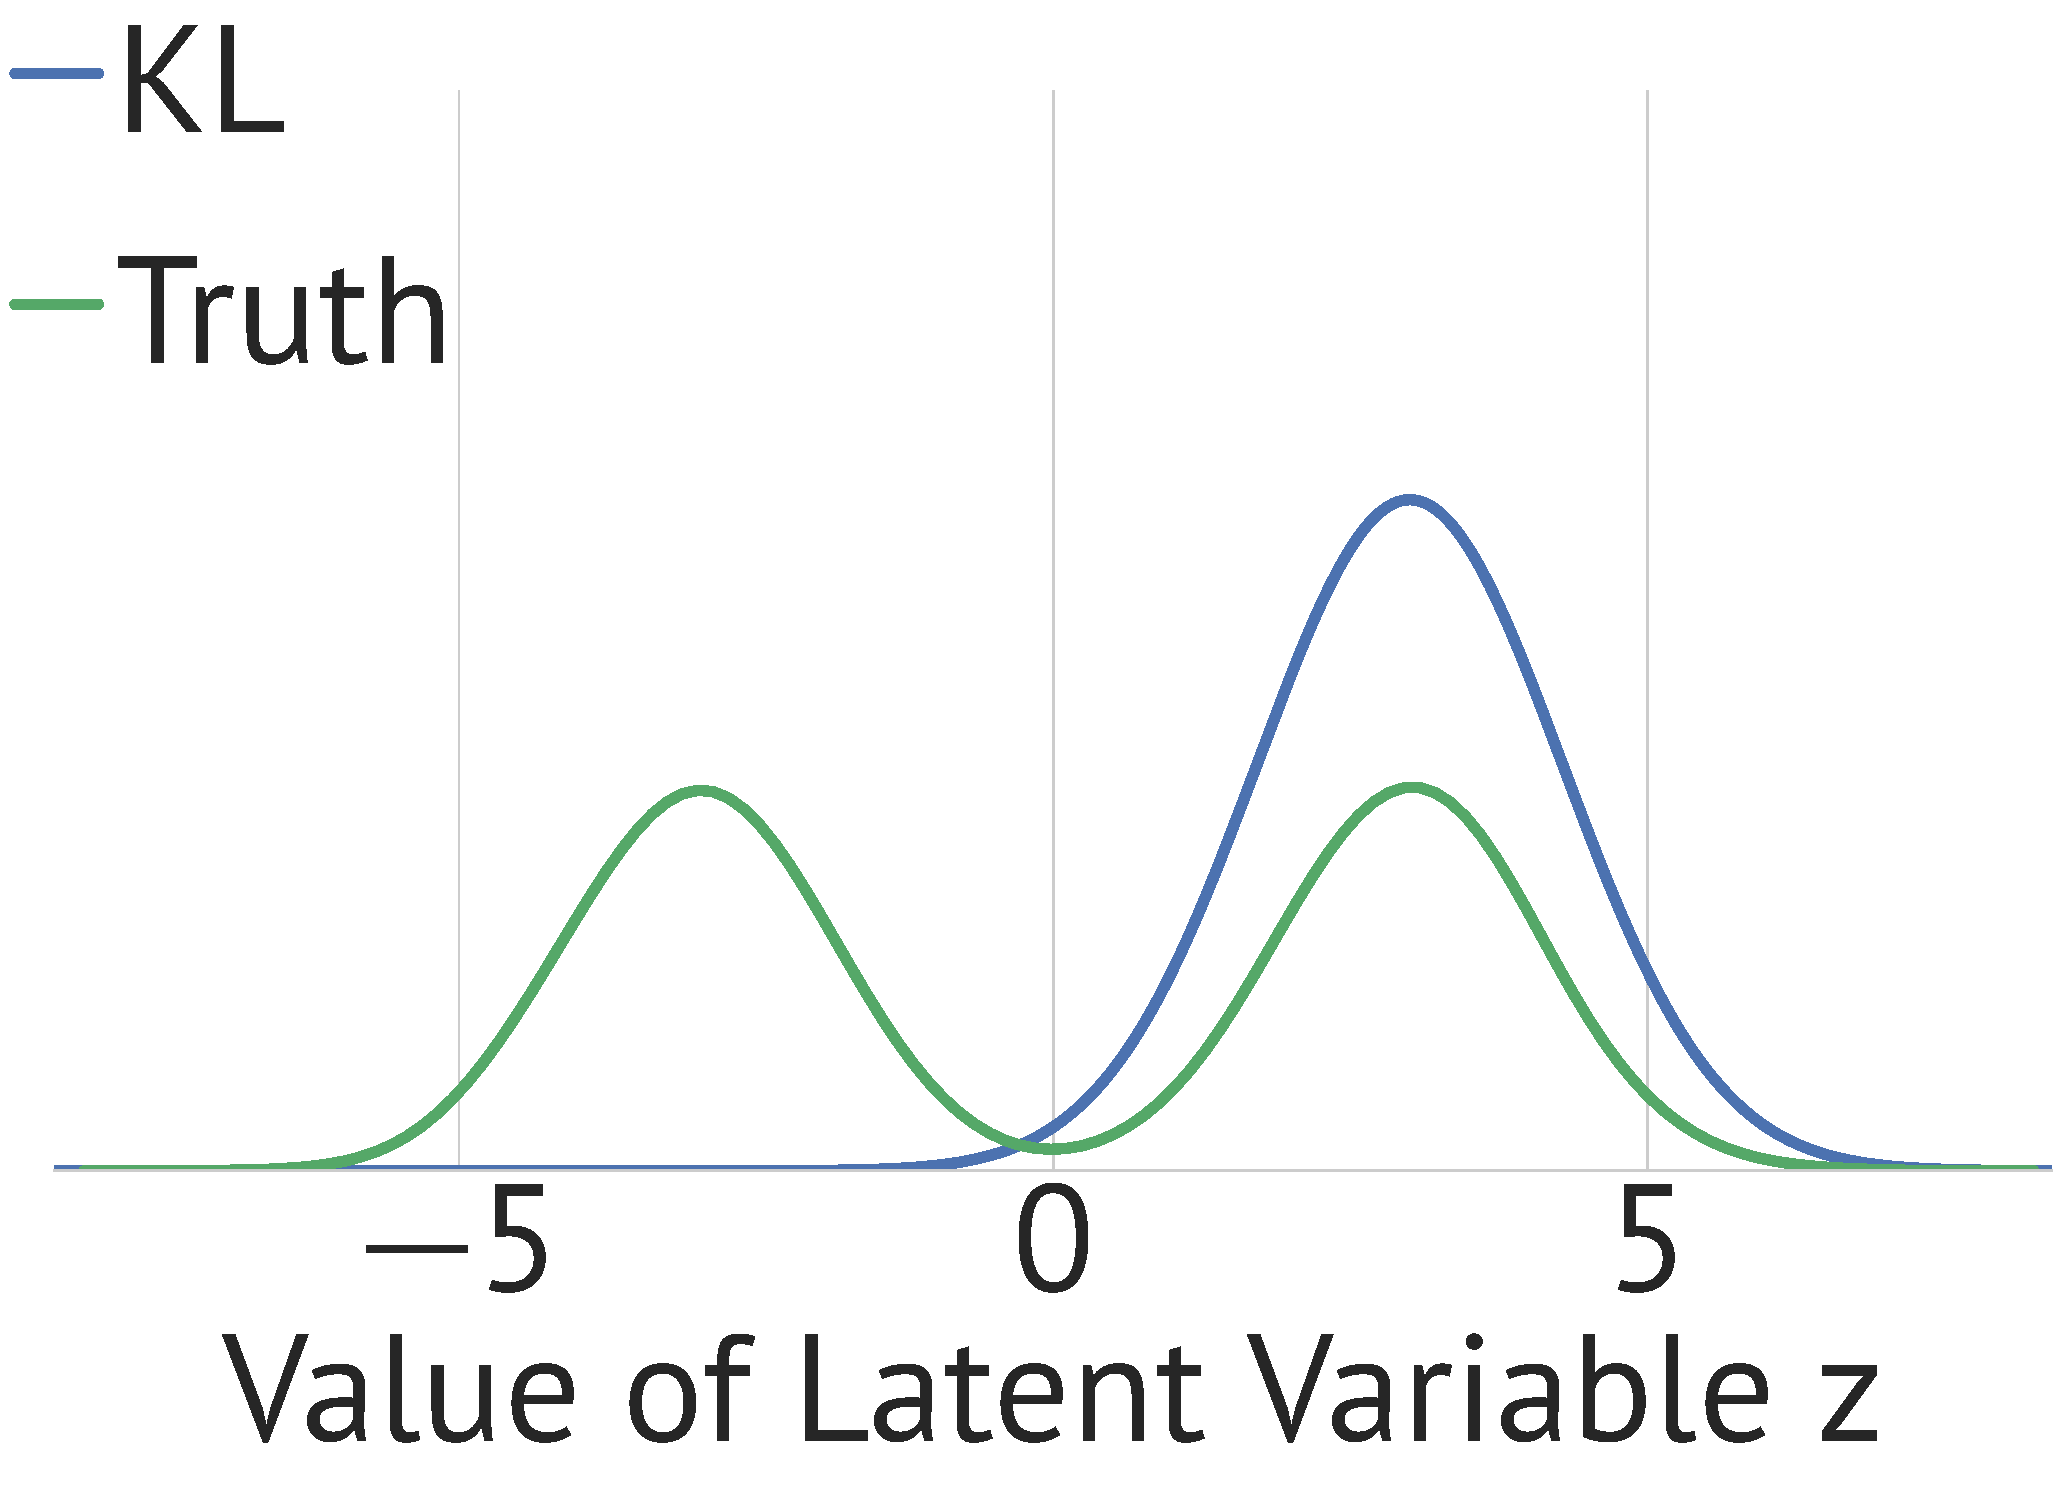
\includegraphics[trim=0 0 0 0, width=\linewidth]{fig/density_KL}
\end{subfigure}
\begin{subfigure}{0.23\textwidth}
  \centering
  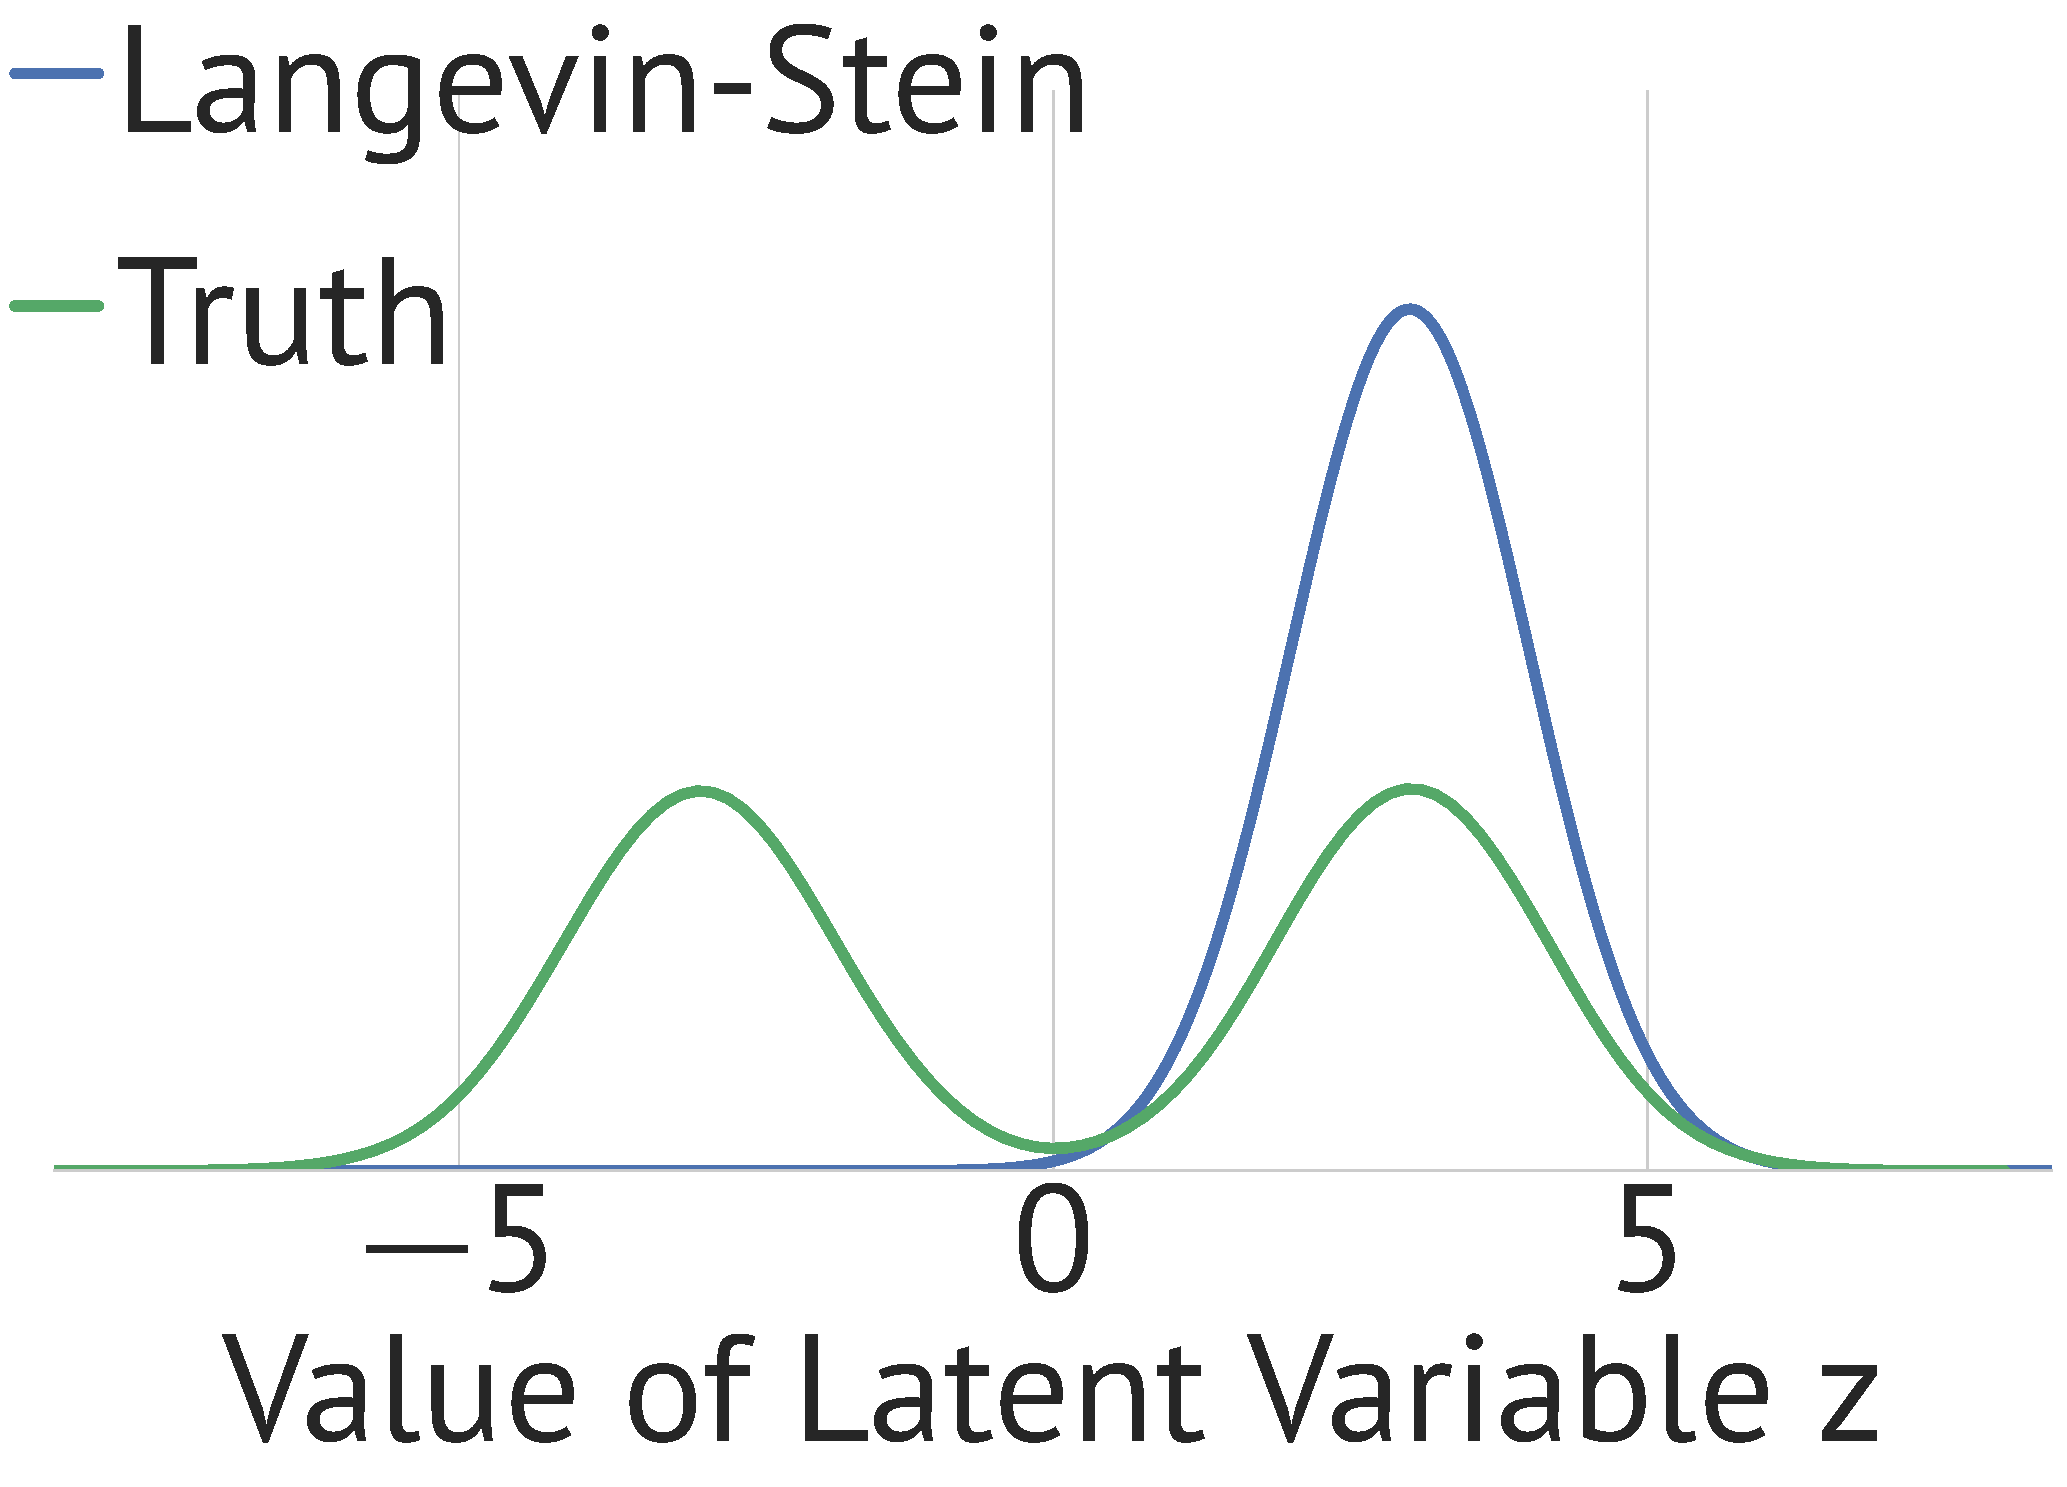
\includegraphics[trim=0 0 0 0, width=\linewidth]{fig/density_Lang-Stein}
\end{subfigure}
\begin{subfigure}{0.23\textwidth}
    \centering
   \includegraphics[trim=0 0 0 0, width=\linewidth]{{"fig/density_Variational Program"}}
\end{subfigure}
\caption{The true posterior is a mixture of two Gaussians, in green. We approximate it with
  a Gaussian using two operators (in blue). The density on the far
  right is a variational program given in~\Cref{eq:toy_var_prog} and
  using the Langevin-Stein operator; it approximates the truth well.
  The density of the variational program is intractable. We plot a histogram
  of its samples and compare this to the histogram of the true posterior.}
\label{fig:mog}\label{fig:toy}
\end{figure}


\Cref{fig:mog} displays the posterior approximations.  We find that the \gls{KL}
divergence and \gls{LS} divergence choose a single mode and have
slightly different variances. These operators do not produce good
results because a single Gaussian is a poor approximation to the
mixture. The remaining distribution in~\Cref{fig:mog} comes from the
toy variational program described by~\Cref{eq:toy_var_prog} with the
\gls{LS} operator.  Because this program
captures different distributions for the positive and negative half of the
real line, it is able to capture the posterior.

In general, the choice of an objective balances statistical and computational properties of variational inference. We highlight one tradeoff: the \gls{LS} objective admits the use of a variational program; however, the objective is more difficult to optimize than the \gls{KL}.



\subsection{Logistic Factor Analysis}
Logistic factor analysis models binary vectors $\mbx_i$ with a matrix of
parameters $\mbW$ and biases $\mbb$,
\begin{align*}
  \mbz_i &\sim \textrm{Normal}(0, 1) \\
  x_{i,k} &\sim \textrm{Bernoulli}(\sigma(\mbw_k^\top \mbz_i + b_k)),
\end{align*}
where $\mbz_i$ has fixed dimension $K$ and $\sigma$ is the sigmoid
function.  This model captures correlations of the entries in $\mbx_i$
through $\mbW$.






We apply logistic factor analysis to analyze the binarized MNIST data
set~\citep{salakhutdinov2008quantitative},
which contains 28x28 binary pixel images of handwritten digits.
(We set the latent dimensionality to 10.)  We fix the model parameters
to those learned with variational expectation-maximization using the
\gls{KL} divergence, and focus on comparing posterior inferences.

We compare the \gls{KL} operator to the \gls{LS} operator and study
two choices of variational models: a fully factorized Gaussian
distribution and a variational program. The variational program
generates samples by transforming a $K$-dimensional standard normal
input with a two-layer neural network, using rectified linear activation
functions and a hidden size of twice the latent dimensionality. Formally, the variational
program we use generates samples of $\mbz$ as follows:
\begin{align*}
\mbz_0 &\sim \textrm{Normal}(0, I) \\
\mbh_0 &= \textrm{ReLU}({\mbW_0^q}^\top \mbz_0 + \mbb_0^q) \\
\mbh_1 &= \textrm{ReLU}({\mbW_1^q}^\top \mbh_0 + \mbb_1^q) \\
\mbz &= {\mbW_2^q}^\top \mbh_1 + \mbb_2^q.
\end{align*}
The variational parameters are the weights $\mbW^q$ and biases $\mbb^q$.
For $f$, we use a
three-layer neural network with the same hidden size as the
variational program and hyperbolic tangent activations where unit
activations were bounded to have norm two. Bounding the unit norm
bounds the divergence. We used the Adam optimizer~\citep{DBLP:journals/corr/KingmaB14} with learning rates $2 \times 10^{-4}$ for
$f$ and $2 \times 10^{-5}$ for the variational approximation.

\begin{table}[tb]
\centering
\begin{tabular}{lcc}
\toprule
Inference method & Completed data log-likelihood
\\
\midrule
Mean-field Gaussian + \gls{KL} & -59.3 \\
Mean-field Gaussian + \gls{LS} &  -75.3 \\
Variational Program + \gls{LS} & -58.9\\
\bottomrule
\end{tabular}
\vspace{1ex}
\caption{Benchmarks on logistic factor analysis for binarized MNIST.
The same variational approximation with \gls{LS} performs worse than
\gls{KL} on likelihood performance. The variational program with
\gls{LS} performs better without directly optimizing for likelihoods.}
\label{table:mnist}
\vskip -.1in
\end{table}

There is no standard for evaluating generative models and their
inference algorithms~\citep{theis2016note}.
Following
\citet{Rezende:2014}, we consider a missing data problem. We remove
half of the pixels in the test set (at random) and reconstruct them
from a fitted posterior predictive distribution. \Cref{table:mnist}
summarizes the results on 100 test images; we report the
log-likelihood of the completed image. \gls{LS} with the variational
program performs best.  It is followed by \gls{KL} and the simpler
\gls{LS} inference. The \gls{LS} performs better than \gls{KL} even
though the model parameters were learned with \gls{KL}.
